\section{Approximation methodology}\label{learning}

Our methodology is based on equipping the processing pipeline with variable levels of approximation, i.e., configurable approximations, and an approximation engine within a supervisor block (which may contain additional optimisations such as parameter tuning): a block diagram is depicted in Fig. \ref{fig:block_diagram}. Depending on the application and the deployment technology (e.g., CPU, ASIC, FPGA) the nature of approximations varies, but our method is applicable across the entire spectrum. Traditional approximation methods include bit width reduction \cite{mittal2016survey}, memoisation \cite{sinha2016low}, predictive memory access \cite{yazdanbakhsh2016mitigating}, arithmetic re-writes \cite{nepal2016automated}, input-based approximations \cite{raha2016input}, etc.
\par Based on prior knowledge about the data, our approximation engine dynamically monitors the processing pipeline's output, and verifies whether or not the calculations still obey the assumptions about the data. If yes, then it is assumed that current levels of accuracy are still within error bounds: hence, the pipeline can be approximated further. If not, then it is assumed that accuracy has exceeded error bounds, and the level of approximation is reduced. Using this method, it is possible to converge on an approximation strategy that optimises power consumption \textit{in situ}, without access to ground truth. 

\par Our approach is predicated on runtime-configurable levels of approximation. In software solutions running on CPUs and GPUs, this can be achieved through different software versions \cite{vassiliadis2015programming} or through Instruction Set Architecture (ISA) level approximations \cite{venkataramani2013quality}. In bespoke hardware solutions implemented on ASIC or FPGA, through configurable hardware versions which clock- or power-gate accurate circuitry; this is the approach we use on our experiments, which we detail in Section \ref{experiments}.

%\begin{figure}[tb]
%  \centering
%  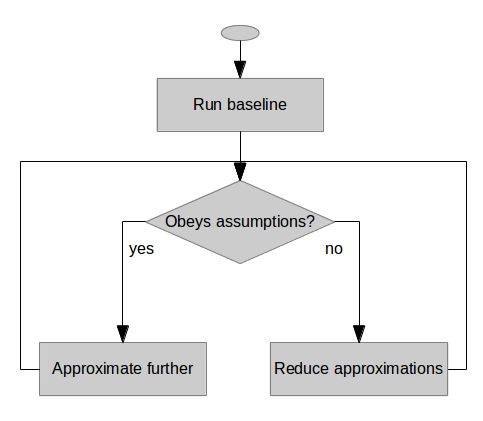
\includegraphics[width=0.7\columnwidth]{img/flowchart.png}
%  \caption{Approximation engine's runtime behaviour.}
%  \label{fig:flowchart}
%\end{figure}
